\documentclass[aspectratio=169,11pt,table]{beamer}
\usepackage{../assets/ccde-beamer}

%% ---------- Metadatos (plantilla canónica: \date{} siempre vacío) ----------
\renewcommand{\ccdefootlabel}{CCDE -- K-Nearest Neighbors (KNN)}
\title{K-Nearest Neighbors (KNN)}
\subtitle{Aprendizaje basado en instancias, métricas y regiones locales}
\author{Círculo de Ciencia de Datos y Econometría}
\date{}

\begin{document}


% ================================================================
% PORTADA OFICIAL CCDE (IDÉNTICA A SVM Y ÁRBOLES)
% ================================================================
% Portada canónica (diseño en assets/ccde-beamer.sty, sin fecha)
\ccdeportada{K-Nearest Neighbors (KNN)}{Aprendizaje basado en instancias, métricas y regiones locales}{KNN}


% ================================================================
% AGENDA / MAPA DE LA PRESENTACIÓN
% ================================================================
\begin{frame}{Mapa de la presentación}
\begin{columns}[T,onlytextwidth]
\begin{column}{0.57\textwidth}
{\small\tableofcontents}
\end{column}
\begin{column}{0.39\textwidth}
\begin{keybox}
\textbf{Pregunta guía}\\[0.14cm]
¿Cómo puede un algoritmo clasificar o predecir sin asumir una función paramétrica global, aprendiendo directamente de la geometría local de los datos?
\end{keybox}
\vspace{0.16cm}
\begin{ccdebox}
\small
\textbf{Fuentes principales}\\
James et al. (ISLR, cap. 2 y 4); Hastie et al. (ESL, cap. 13); Géron (2022, cap. 3).\\[0.12cm]
\textbf{Aplicación práctica}\\
Python + scikit-learn con Pipeline reproducible.
\end{ccdebox}
\end{column}
\end{columns}
\end{frame}

% ================================================================
% SECCIONES MODULARES
% ================================================================
\section{Fundamentos e Intuición de KNN}

% ================================================================
\begin{frame}{¿Qué es K-Nearest Neighbors (KNN)?}
\begin{columns}[T,onlytextwidth]
\begin{column}{0.54\textwidth}
\begin{ccdebox}
\footnotesize
\textbf{K-Nearest Neighbors (KNN)} es un algoritmo supervisado \textbf{no paramétrico} y \textbf{basado en instancias}.
\end{ccdebox}

\vspace{0.05cm}
\begin{itemize}\setlength{\itemsep}{0.10em}
  \footnotesize
  \item \textbf{Sin parámetros globales}: no calcula un vector $\beta$.
  \item \textbf{Lazy learning}: memoriza el conjunto de entrenamiento.
  \item \textbf{Fronteras locales}: aproxima relaciones no lineales.
\end{itemize}

\vspace{0.06cm}
\begin{keybox}
\footnotesize \textbf{Regla de decisión}: la predicción para $x_0$ se obtiene consultando el vecindario local $\mathcal{N}_k(x_0)$.
\end{keybox}
\end{column}

\begin{column}{0.43\textwidth}
\centering
\begin{tikzpicture}[scale=0.68]
  \draw[step=1cm,ccdeice!70,very thin] (-2,-2) grid (2,2);
  
  \fill[ccdeaccent] (-1.2,0.8) circle (2.6pt) node[above left=1pt,font=\tiny\bfseries,text=ccdemid]{Clase A};
  \fill[ccdeaccent] (-0.7,1.3) circle (2.6pt);
  \fill[ccdeaccent] (-1.4,-0.4) circle (2.6pt);
  \fill[ccdeaccent] (-0.4,0.6) circle (2.6pt);
  \fill[ccdeaccent] (-0.8,-0.2) circle (2.6pt);

  \fill[warn] (1.1,-0.7) circle (2.6pt) node[below right=1pt,font=\tiny\bfseries,text=warn]{Clase B};
  \fill[warn] (0.6,-1.2) circle (2.6pt);
  \fill[warn] (1.4,0.3) circle (2.6pt);
  \fill[warn] (0.4,-0.5) circle (2.6pt);
  \fill[warn] (1.0,-1.4) circle (2.6pt);

  \node[draw=ccdenavy,fill=white,circle,inner sep=2.5pt,line width=1.2pt] (x0) at (0,0) {};
  \fill[ccdenavy] (0,0) circle (1.2pt);
  \node[above=2.5pt of x0,font=\scriptsize\bfseries,text=ccdenavy] {$x_0$};

  \draw[ccdemid,thick,dashed] (x0) circle (0.95cm);
  \node[below=0.97cm of x0,font=\tiny\bfseries,text=ccdemid]{$\mathcal{N}_3(x_0)$};

  \draw[ccdesky,dotted,line width=0.9pt] (x0) circle (1.55cm);
  \node[above=1.57cm of x0,font=\tiny\bfseries,text=ccdesky]{$\mathcal{N}_5(x_0)$};
\end{tikzpicture}
\end{column}
\end{columns}

\vspace{0.10cm}
\source{James et al. (2013), cap. 2; Hastie et al. (2009), cap. 13.}
\end{frame}

% ================================================================
\begin{frame}{Paradigma: Modelos Paramétricos vs. Basados en Instancias}
\begin{columns}[T,onlytextwidth]
\begin{column}{0.48\textwidth}
\begin{contrastbox}{ccdemid}{Enfoque Paramétrico}
\footnotesize
\textbf{Ejemplos:} Regresión lineal, Logit, LDA.
\begin{itemize}\setlength{\itemsep}{0.12em}
  \item Asume forma funcional global explícita:
  \[ f(X) = \beta_0 + \sum_{j=1}^p \beta_j X_j \]
  \item \textbf{Entrenamiento:} intensivo (optimización).
  \item \textbf{Inferencia:} instantánea con $\hat{\beta}$.
  \item \textbf{Riesgo:} sesgo por mala especificación.
\end{itemize}
\end{contrastbox}
\end{column}

\begin{column}{0.48\textwidth}
\begin{contrastbox}{ccdeaccent}{Enfoque No Paramétrico (KNN)}
\footnotesize
\textbf{Ejemplos:} KNN, Splines, Kernel regression.
\begin{itemize}\setlength{\itemsep}{0.12em}
  \item Sin estructura funcional previa:
  \[ \hat{f}(x_0) = \mathrm{Agreg}(\{y_i : x_i \in \mathcal{N}_k(x_0)\}) \]
  \item \textbf{Entrenamiento:} pasivo (memorización).
  \item \textbf{Inferencia:} costo $O(N \cdot p)$ por consulta.
  \item \textbf{Riesgo:} alta varianza en alta dimensión.
\end{itemize}
\end{contrastbox}
\end{column}
\end{columns}
\source{Géron (2022), cap. 3; James et al. (2013), cap. 2.}
\end{frame}

\section{Formulación Matemática de KNN}

% ================================================================
\begin{frame}{KNN en Clasificación: Voto Mayoritario y Probabilidad}
\begin{columns}[T,onlytextwidth]
\begin{column}{0.48\textwidth}
\begin{ccdebox}
\textbf{Definición de Vecindad Local}\\[0.06cm]
Sea $\mathcal{D} = \{(x_i, y_i)\}_{i=1}^N$ y $x_0$ un punto de consulta. $\mathcal{N}_k(x_0)$ contiene los $k$ puntos más cercanos a $x_0$ según $d(\cdot, \cdot)$.
\end{ccdebox}

\vspace{0.08cm}
\begin{contrastbox}{ccdemid}{Probabilidad a Posteriori}
\footnotesize
Frecuencia empírica en el vecindario para la clase $c \in \mathcal{C}$:
\[
\widehat{P}(Y = c \mid X = x_0) = \frac{1}{k} \sum_{i \in \mathcal{N}_k(x_0)} \mathbb{I}(y_i = c)
\]
\end{contrastbox}
\end{column}

\begin{column}{0.48\textwidth}
\begin{contrastbox}{ccdeaccent}{Regla de Voto Mayoritario}
\footnotesize
Asigna la clase con mayor soporte en $\mathcal{N}_k(x_0)$:
\[
\hat{y}(x_0) = \arg\max_{c \in \mathcal{C}} \sum_{i \in \mathcal{N}_k(x_0)} \mathbb{I}(y_i = c)
\]
\end{contrastbox}

\vspace{0.08cm}
\begin{keybox}
\scriptsize
\textbf{Teorema de Cover y Hart (1967)}:\\
Cuando $N \to \infty$, la tasa de error del 1-NN satisface:
\[ R^* \leq R_{1\text{-NN}} \leq 2R^*(1 - R^*) \]
donde $R^*$ es el error del clasificador óptimo de Bayes.
\end{keybox}
\end{column}
\end{columns}
\source{Cover \& Hart (1967); James et al. (2013), cap. 2.}
\end{frame}

% ================================================================
\begin{frame}{KNN en Regresión y Ponderación por Distancia}
\begin{columns}[T,onlytextwidth]
\begin{column}{0.48\textwidth}
\begin{contrastbox}{ccdemid}{KNN Regresión Estándar}
\footnotesize
Para $y_i \in \mathbb{R}$, media local de vecinos:
\[
\hat{f}(x_0) = \frac{1}{k} \sum_{i \in \mathcal{N}_k(x_0)} y_i
\]
\begin{itemize}\setlength{\itemsep}{0.06em}
  \item Función escalonada por tramos.
  \item Ponderación uniforme ($1/k$) en $\mathcal{N}_k(x_0)$.
\end{itemize}
\end{contrastbox}
\end{column}

\begin{column}{0.48\textwidth}
\begin{contrastbox}{ccdeaccent}{Ponderación por Distancia}
\footnotesize
Mayor influencia a observaciones próximas:
\[
w_i = \frac{1}{d(x_0, x_i)^p}, \quad \hat{f}(x_0) = \frac{\sum_{i \in \mathcal{N}_k} w_i y_i}{\sum_{i \in \mathcal{N}_k} w_i}
\]
\begin{itemize}\setlength{\itemsep}{0.06em}
  \item Genera fronteras y ajustes suaves.
  \item Atenúa el impacto de puntos lejanos.
\end{itemize}
\end{contrastbox}
\end{column}
\end{columns}

\vspace{0.06cm}
\begin{ccdebox}
\scriptsize \textbf{Interpretación}: KNN ponderado equivale a un \textbf{estimador de Nadaraya-Watson} con ancho de banda adaptativo a la distancia del $k$-ésimo vecino.
\end{ccdebox}
\source{Hastie, Tibshirani \& Friedman (2009), cap. 6 y 13.}
\end{frame}

\section{Métricas de Distancia y Geometría}

% ================================================================
\begin{frame}{Métricas de Distancia en $\mathbb{R}^p$}
\footnotesize
\begin{center}
\renewcommand{\arraystretch}{1.15}
\begin{tabular}{llp{6.3cm}}
\toprule
\textbf{\textcolor{ccdenavy}{Métrica}} & \textbf{\textcolor{ccdenavy}{Fórmula}} & \textbf{\textcolor{ccdenavy}{Propiedades y Uso Práctico}} \\
\midrule
\textbf{Euclidiana} ($L_2$) & $\sqrt{\sum_{j=1}^p (x_j - z_j)^2}$ & Distancia geodésica estándar en $\mathbb{R}^p$. Asume isotropía. \\
\textbf{Manhattan} ($L_1$) & $\sum_{j=1}^p |x_j - z_j|$ & Distancia taxicab. Más robusta ante valores atípicos que $L_2$. \\
\textbf{Minkowski} ($L_q$) & $\left(\sum_{j=1}^p |x_j - z_j|^q\right)^{\frac{1}{q}}$ & Generaliza $L_1$ ($q=1$) y $L_2$ ($q=2$). \\
\textbf{Chebyshev} ($L_\infty$) & $\max_{j} |x_j - z_j|$ & Dominada por la dimensión de mayor discrepancia. \\
\textbf{Hamming} & $\sum_{j=1}^p \mathbb{I}(x_j \neq z_j)$ & Para variables binarias o categóricas discretas. \\
\bottomrule
\end{tabular}
\end{center}

\vspace{0.06cm}
\begin{keybox}
\footnotesize \textbf{Conclusión}: La métrica define formalmente el concepto de vecindad. Modificar la distancia altera el orden relativo de los vecinos y puede cambiar la predicción manteniendo $k$ fijo.
\end{keybox}
\source{Géron (2022), cap. 3; Hastie et al. (2009), cap. 13.}
\end{frame}

% ================================================================
\begin{frame}{Geometría de Bolas Unitarias en 2D}
\begin{columns}[c,onlytextwidth]
\begin{column}{0.62\textwidth}
\centering
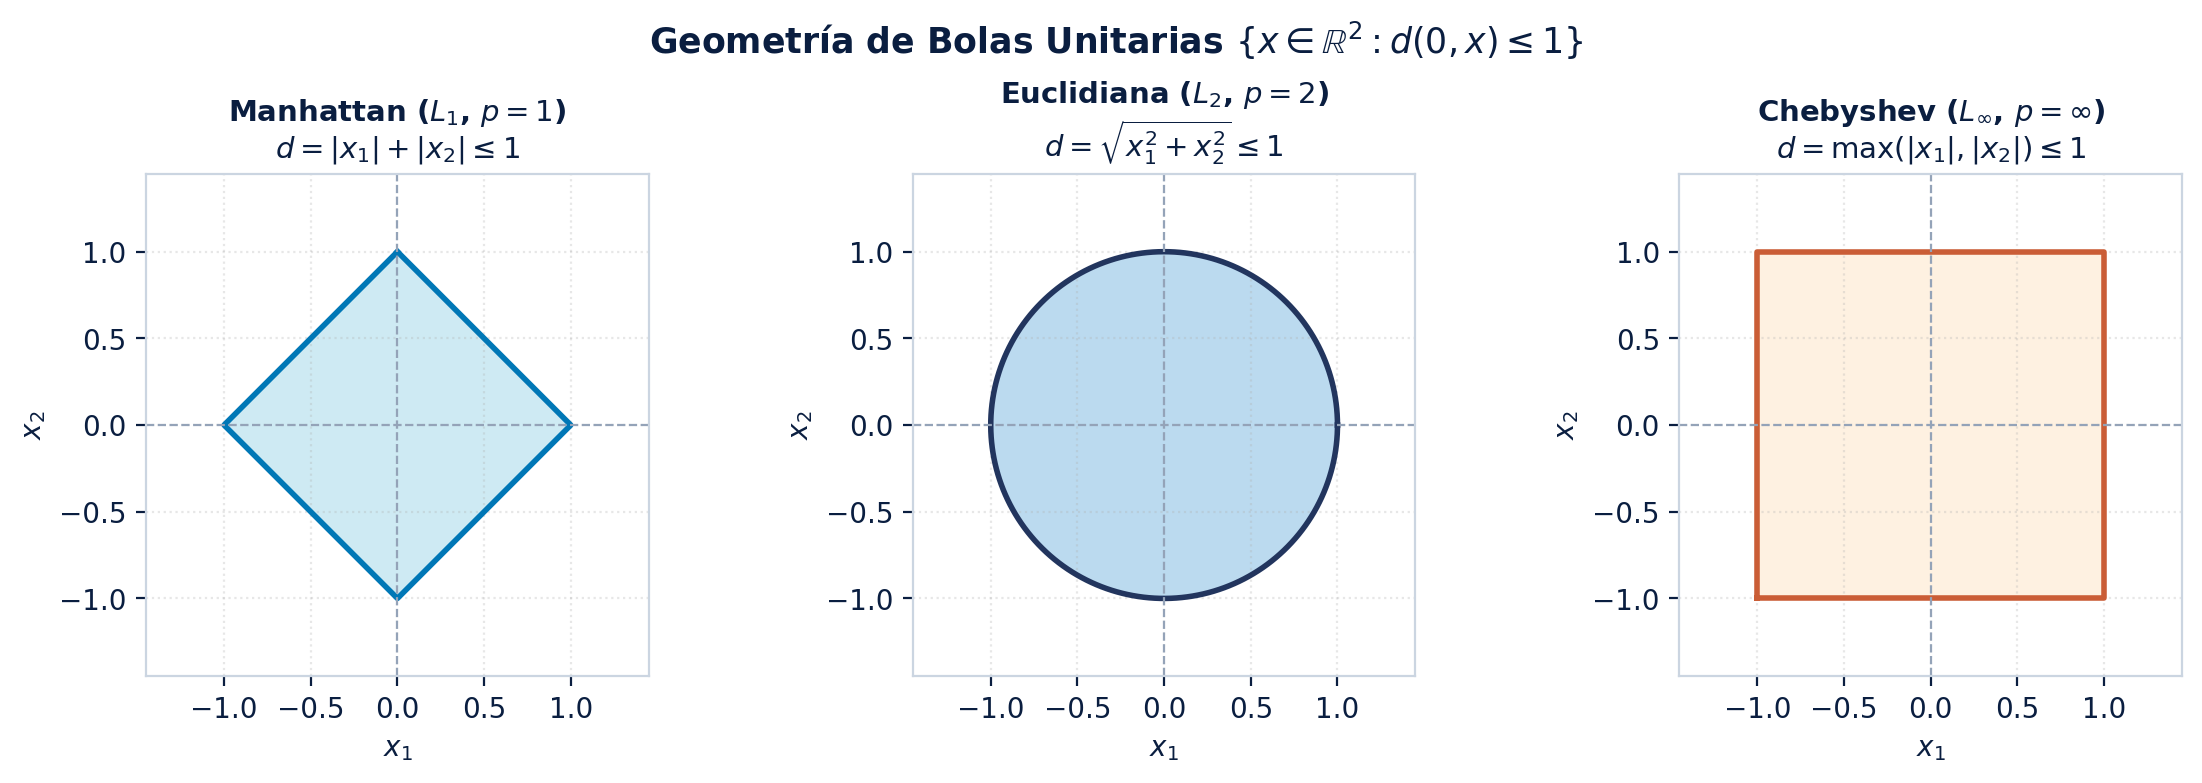
\includegraphics[width=\linewidth]{fig_distancias_knn.png}
\end{column}

\begin{column}{0.36\textwidth}
\begin{contrastbox}{ccdemid}{Lectura Geométrica}
\footnotesize
Bolas unitarias $\{x : d(0, x) \le 1\}$:
\begin{itemize}\setlength{\itemsep}{0.18em}
  \item \textbf{Manhattan ($L_1$):} rombo orientado a $45^\circ$.
  \item \textbf{Euclidiana ($L_2$):} circunferencia perfecta.
  \item \textbf{Chebyshev ($L_\infty$):} cuadrado ortogonal.
\end{itemize}
\end{contrastbox}

\vspace{0.10cm}
\begin{ccdebox}
\scriptsize
\textbf{Efecto en la frontera}: al pasar de $L_2$ a $L_1$ o $L_\infty$, las fronteras de decisión se vuelven poligonales.
\end{ccdebox}
\end{column}
\end{columns}
\source{Figura reproducible generada con Python scikit-learn y matplotlib (CCDE).}
\end{frame}

\section{Escalamiento e Hiperparámetros}

% ================================================================
\begin{frame}{Por Qué el Escalamiento es Crítico en KNN}
\footnotesize
\begin{columns}[T,onlytextwidth]
\begin{column}{0.54\textwidth}
\begin{ccdebox}
Como KNN mide distancias absolutas en $\mathbb{R}^p$, variables con mayor escala numérica dominan arbitrariamente la cercanía.
\end{ccdebox}

\vspace{0.06cm}
\begin{itemize}\setlength{\itemsep}{0.12em}
  \item \textbf{Ejemplo}: Ingreso mensual ($\$1\,000$ a $\$20\,000$) vs. Edad ($18$ a $80$).
  \item Diferencia de $\$100$ eclipsa totalmente $40$ años de edad.
  \item \textbf{Efecto}: la distancia ignora las variables de menor escala.
\end{itemize}
\end{column}

\begin{column}{0.44\textwidth}
\centering
\begin{tikzpicture}[scale=0.72]
  \draw[->,ccdenavy,line width=0.8pt] (0,0) -- (4.0,0) node[below,font=\tiny]{Ingreso};
  \draw[->,ccdenavy,line width=0.8pt] (0,0) -- (0,3.0) node[left,font=\tiny]{Edad};
  
  % Elipse deformada amplia
  \draw[warn,thick,dashed] (2.0,1.55) ellipse (1.70cm and 0.50cm);
  \node[warn,font=\tiny\bfseries,align=center] at (2.0,2.35) {Vecindad deformada};

  % Punto de consulta x0 nítido y legible con diana
  \node (x0) at (2.0,1.55) [draw=ccdenavy,fill=white,circle,inner sep=2.4pt,line width=1.2pt] {};
  \fill[ccdenavy] (2.0,1.55) circle (1.2pt);
  \node[left=3.5pt of x0,font=\scriptsize\bfseries,text=ccdenavy] {$x_0$};

  % Puntos en la misma elipse
  \fill[ccdeaccent] (0.85,1.55) circle (2.2pt);
  \fill[ccdeaccent] (3.15,1.55) circle (2.2pt);

  % Punto descartado
  \fill[purplex] (2.0,0.50) circle (2.2pt) node (pout) {};
  \node[right=2.5pt of pout,font=\tiny,text=purplex,align=left]{Descartado a pesar\\de ser cercano};
\end{tikzpicture}

\vspace{0.08cm}
\begin{contrastbox}{okgreen}{Solución con StandardScaler}
Estandarizar ($z_j = \frac{x_j - \mu_j}{\sigma_j}$) en un \texttt{Pipeline} para evitar fuga de datos (\textit{leakage}).
\end{contrastbox}
\end{column}
\end{columns}
\source{Géron (2022), cap. 3; James et al. (2013), cap. 4.}
\end{frame}

% ================================================================
\begin{frame}{El Papel de $k$: Trade-Off Sesgo--Varianza}
\begin{columns}[T,onlytextwidth]
\begin{column}{0.48\textwidth}
\begin{contrastbox}{warn}{k Pequeño: Flexibilidad}
\scriptsize
\textbf{Bajo sesgo / Alta varianza ($k=1$)}
\begin{itemize}\setlength{\itemsep}{0.10em}
  \item Reproduce fielmente el training set.
  \item Frontera fragmentada, sensible a anomalías.
\end{itemize}
\end{contrastbox}

\vspace{0.08cm}
\begin{contrastbox}{ccdemid}{k Grande: Regularización}
\scriptsize
\textbf{Alto sesgo / Baja varianza ($k \to N$)}
\begin{itemize}\setlength{\itemsep}{0.10em}
  \item Fronteras excesivamente suaves.
  \item Predice la clase mayoritaria global.
\end{itemize}
\end{contrastbox}
\end{column}

\begin{column}{0.49\textwidth}
\centering
\begin{tikzpicture}[scale=0.74]
  \draw[->,ccdenavy,line width=0.8pt] (0,0) -- (4.2,0) node[right,font=\tiny]{$1/k$};
  \draw[->,ccdenavy,line width=0.8pt] (0,0) -- (0,2.9) node[left,font=\tiny]{Error};

  \draw[okgreen,thick] (0.4,2.3) to[out=-40,in=175] (3.8,0.3);
  \node[okgreen,font=\tiny\bfseries] at (3.8,0.55) {Train};

  \draw[warn,thick] (0.4,2.5) to[out=-50,in=180] (2.0,1.1) to[out=0,in=215] (3.8,2.4);
  \node[warn,font=\tiny\bfseries] at (3.8,2.65) {Test};

  \draw[ccdemid,dashed,line width=0.8pt] (2.0,0) -- (2.0,1.1);
  \node[below=1pt,font=\tiny\bfseries,text=ccdemid] at (2.0,0) {$k^*$ óptimo};
  \fill[ccdemid] (2.0,1.1) circle (2pt);
\end{tikzpicture}

\vspace{0.06cm}
\begin{keybox}
\footnotesize \textbf{Regla}: el hiperparámetro $k$ se optimiza mediante \textbf{validación cruzada} (CV).
\end{keybox}
\end{column}
\end{columns}
\source{Hastie, Tibshirani \& Friedman (2009), cap. 2 y 13.}
\end{frame}

% ================================================================
\begin{frame}{Evolución de las Regiones de Decisión según $k$}
\centering
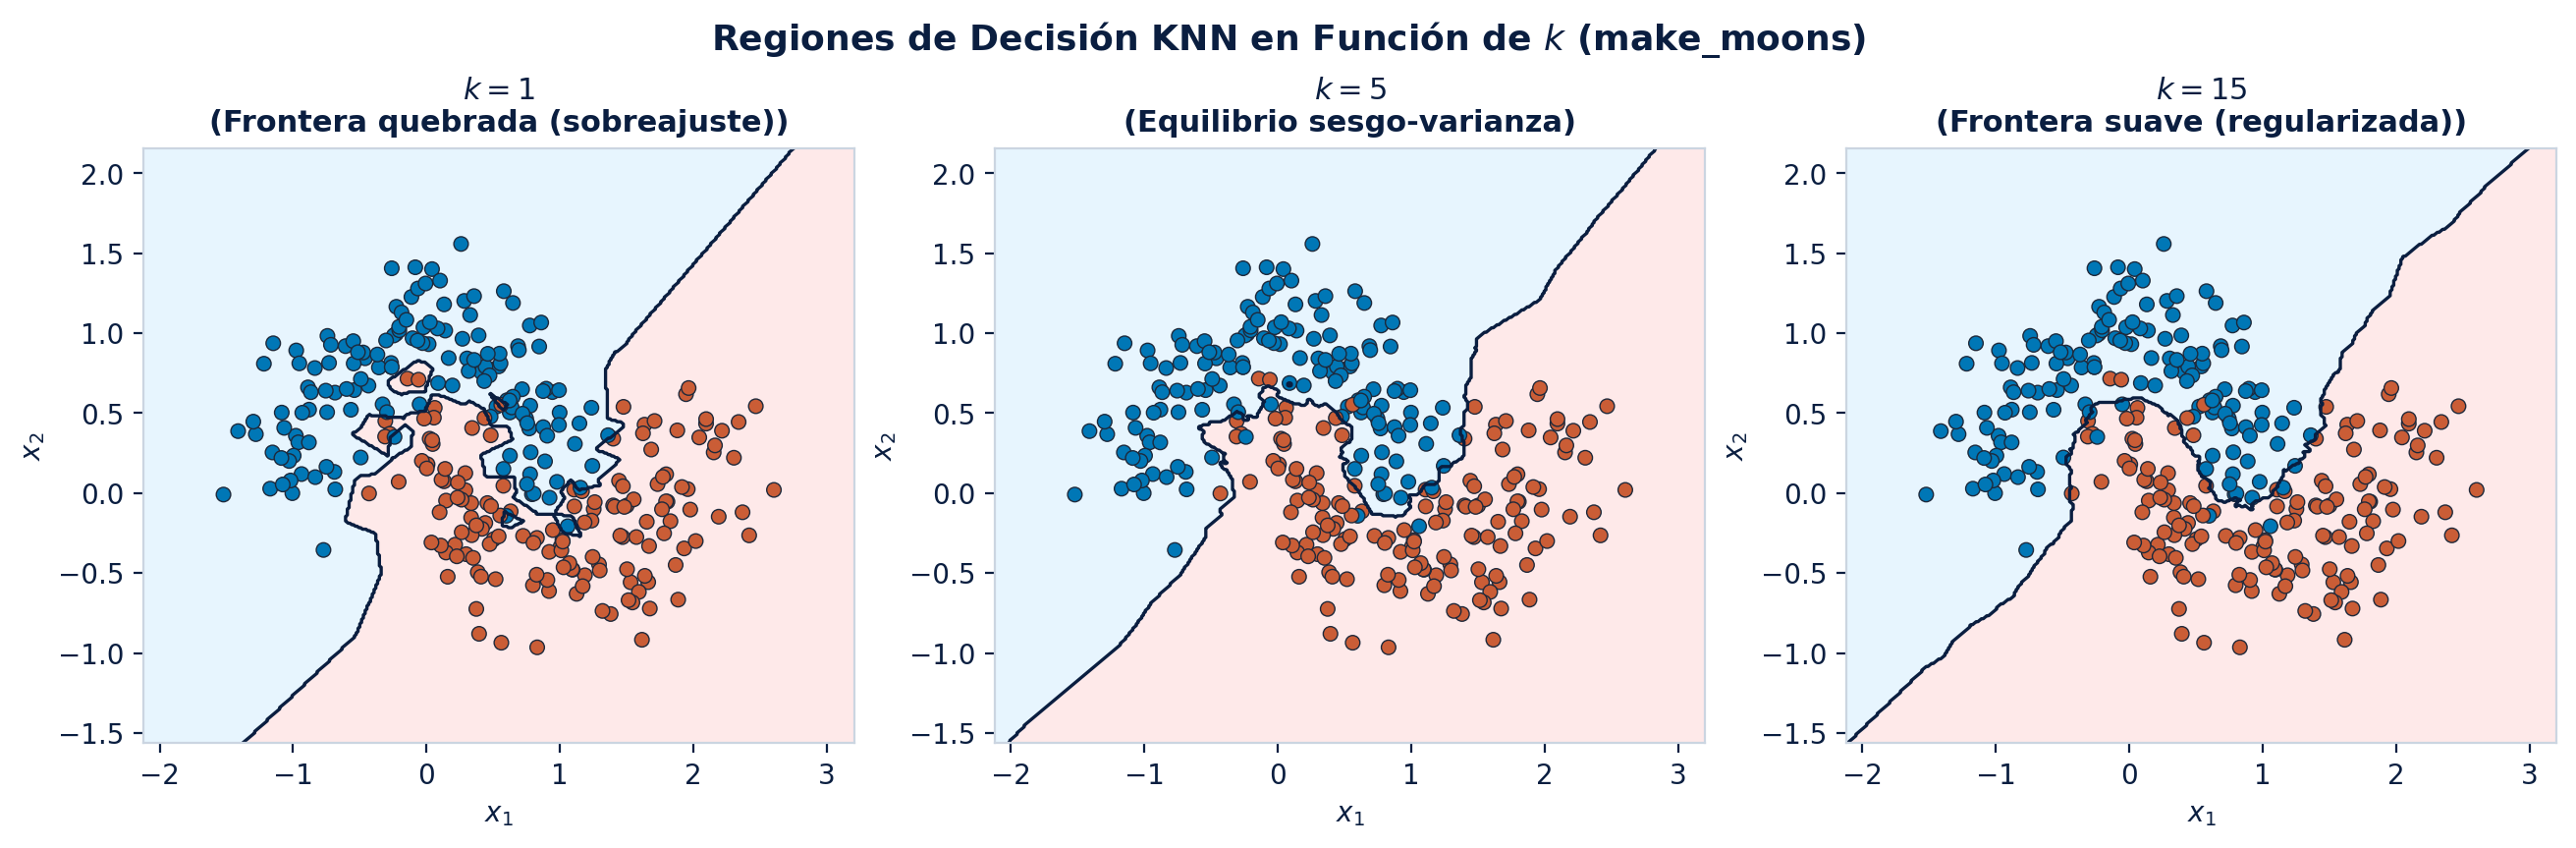
\includegraphics[width=0.90\linewidth]{fig_knn_regions.png}

\vspace{-0.05cm}
\begin{columns}[T,onlytextwidth]
\begin{column}{0.32\textwidth}
\begin{ccdebox}
\scriptsize
\textbf{$k = 1$ (Sobreajuste):}\\
Frontera hiperflexible; islas espurias alrededor de puntos ruidosos.
\end{ccdebox}
\end{column}

\begin{column}{0.32\textwidth}
\begin{keybox}
\scriptsize
\textbf{$k = 5$ (Balance Óptimo):}\\
Captura la curvatura no lineal de las lunas respetando la estructura.
\end{keybox}
\end{column}

\begin{column}{0.32\textwidth}
\begin{ccdebox}
\scriptsize
\textbf{$k = 15$ (Regularizado):}\\
Frontera suave y estable; reduce la varianza minimizando el sobreajuste.
\end{ccdebox}
\end{column}
\end{columns}
\source{Figura generada con scikit-learn (\texttt{make\_moons}) y \texttt{KNeighborsClassifier}.}
\end{frame}

\section{Maldición de la Dimensionalidad y Complejidad}

% ================================================================
\begin{frame}{La Maldición de la Dimensionalidad (\textit{Curse of Dimensionality})}
\begin{columns}[T,onlytextwidth]
\begin{column}{0.50\textwidth}
\begin{contrastbox}{warn}{El Hipervolumen Vacío}
\scriptsize
En $[0, 1]^p$, capturar una fracción $r \in (0, 1)$ del volumen total exige una arista local:
\[
e_p(r) = r^{\frac{1}{p}}
\]
\begin{itemize}\setlength{\itemsep}{0.05em}
  \item $p = 1$: $e_1(0.10) = 0.10$ ($10\%$ del rango).
  \item $p = 10$: $e_{10}(0.10) \approx 0.80$ ($80\%$ del rango).
  \item $p = 100$: $e_{100}(0.10) \approx 0.98$ ($98\%$ del rango).
\end{itemize}
\end{contrastbox}
\end{column}

\begin{column}{0.48\textwidth}
\begin{ccdebox}
\scriptsize
\textbf{Consecuencia Teórica para KNN:}\\[0.05cm]
En alta dimensión, una vecindad de $k$ puntos \textbf{deja de ser local}: abarca casi todo el espacio muestral.
\end{ccdebox}

\vspace{0.06cm}
\begin{keybox}
\scriptsize
\textbf{Equidistancia Asintótica}:
\[
\lim_{p \to \infty} \frac{d_{\max} - d_{\min}}{d_{\min}} = 0
\]
Todos los puntos quedan aproximadamente a la misma distancia, diluyendo el concepto de cercanía.
\end{keybox}
\end{column}
\end{columns}
\source{Hastie, Tibshirani \& Friedman (2009), cap. 2; Donoho (2000).}
\end{frame}

% ================================================================
\begin{frame}{Estructuras de Indexación y Complejidad}
\begin{columns}[T,onlytextwidth]
\begin{column}{0.48\textwidth}
\begin{ccdebox}
\scriptsize
\textbf{Algoritmos de Búsqueda}
\begin{itemize}\setlength{\itemsep}{0.08em}
  \item \textbf{Fuerza Bruta (\texttt{brute})}: $O(N \cdot p)$ por consulta; evalúa todas las distancias.
  \item \textbf{KD-Tree (\texttt{kd\_tree})}: Partición ortogonal; eficiente con $p \le 20$ ($O(p \log N)$).
  \item \textbf{Ball-Tree (\texttt{ball\_tree})}: Hiperesferas anidadas; óptimo para métricas no euclidianas.
\end{itemize}
\end{ccdebox}
\end{column}

\begin{column}{0.48\textwidth}
\begin{contrastbox}{ccdemid}{Balance Metodológico}
\scriptsize
\textbf{Fortalezas}:
\begin{itemize}\setlength{\itemsep}{0.05em}
  \item Intuitivo y no paramétrico.
  \item Excelente \textit{baseline} no lineal.
  \item Extensión natural a multiclase.
\end{itemize}
\textbf{Limitaciones}:
\begin{itemize}\setlength{\itemsep}{0.05em}
  \item Latencia en inferencia ($O(N \cdot p)$).
  \item Sensible a variables irrelevantes.
  \item Almacenamiento continuo de datos.
\end{itemize}
\end{contrastbox}
\end{column}
\end{columns}
\source{Bentley (1975); Omohundro (1989); scikit-learn documentation.}
\end{frame}

\section{Implementación Reproducible en Python}

% ================================================================
\begin{frame}[fragile]{Pipeline con Scikit-Learn: Prevención de Data Leakage}
\begin{columns}[T,onlytextwidth]
\begin{column}{0.58\textwidth}
\begin{lstlisting}[style=ccdepython]
from sklearn.datasets import load_breast_cancer
from sklearn.model_selection import train_test_split
from sklearn.pipeline import Pipeline
from sklearn.preprocessing import StandardScaler
from sklearn.neighbors import KNeighborsClassifier

X, y = load_breast_cancer(return_X_y=True)
X_tr, X_te, y_tr, y_te = train_test_split(
    X, y, test_size=0.25, stratify=y, random_state=42
)

# Pipeline estricto: escalamiento + estimador
pipe = Pipeline([
    ("scaler", StandardScaler()),
    ("knn", KNeighborsClassifier())
])
\end{lstlisting}
\end{column}

\begin{column}{0.40\textwidth}
\begin{keybox}
\textbf{Arquitectura Pipeline}:
\begin{itemize}\setlength{\itemsep}{0.15em}
  \footnotesize
  \item Aplica $\mu$ y $\sigma$ aprendidos \textbf{solo en el pliegue de entrenamiento}.
  \item Evita fuga de información (\textit{data leakage}) al test/validación.
  \item Facilita la reproducibilidad integral del flujo.
\end{itemize}
\end{keybox}

\vspace{0.10cm}
\begin{ccdebox}
\scriptsize
\textbf{Dataset}: Breast Cancer Wisconsin (569 obs., 30 features numéricas).
\end{ccdebox}
\end{column}
\end{columns}
\source{Script reproducible \texttt{codigo\_demo\_knn.py} (CCDE).}
\end{frame}

% ================================================================
\begin{frame}[fragile]{Búsqueda de Hiperparámetros con GridSearchCV}
\begin{columns}[T,onlytextwidth]
\begin{column}{0.58\textwidth}
\begin{lstlisting}[style=ccdepython]
from sklearn.model_selection import GridSearchCV

param_grid = {
    "knn__n_neighbors": [3, 5, 7, 9, 11, 15],
    "knn__weights": ["uniform", "distance"],
    "knn__metric": ["minkowski"],
    "knn__p": [1, 2] # 1: Manhattan, 2: Euclidiana
}

grid = GridSearchCV(
    pipe,
    param_grid=param_grid,
    cv=5,
    scoring="roc_auc",
    n_jobs=-1
)
grid.fit(X_tr, y_tr)
best_knn = grid.best_estimator_
\end{lstlisting}
\end{column}

\begin{column}{0.40\textwidth}
\begin{contrastbox}{ccdemid}{Espacio de Búsqueda}
\footnotesize
\begin{itemize}\setlength{\itemsep}{0.15em}
  \item \textbf{Vecindades ($k$)}: de $3$ a $15$ impares para evitar empates.
  \item \textbf{Ponderación}: uniforme vs inversa a la distancia.
  \item \textbf{Métricas}: norma $L_1$ vs $L_2$.
  \item \textbf{Criterio}: ROC-AUC con 5 pliegues estratificados.
\end{itemize}
\end{contrastbox}
\end{column}
\end{columns}
\source{Pedregosa et al. (2011); scikit-learn documentation.}
\end{frame}

% ================================================================
\begin{frame}{Resultados Empíricos y Matriz de Confusión}
\begin{columns}[T,onlytextwidth]
\begin{column}{0.51\textwidth}
\begin{ccdebox}
\footnotesize
\textbf{Mejor Configuración Encontrada}
\vspace{0.06cm}

\renewcommand{\arraystretch}{1.12}
\begin{tabular*}{\linewidth}{@{\extracolsep{\fill}}l r@{}}
\toprule
\textbf{\textcolor{ccdenavy}{Parámetro / Métrica}} & \textbf{\textcolor{ccdenavy}{Valor}} \\
\midrule
$k$ óptimo (\texttt{n\_neighbors}) & \textbf{15} \\
Ponderación (\texttt{weights}) & \textbf{\texttt{distance}} \\
Métrica & \textbf{Euclidiana ($L_2$)} \\
ROC-AUC CV (5-fold) & \textbf{0.9875} \\
Accuracy en Test & \textbf{96.50\%} \\
ROC-AUC en Test & \textbf{0.9948} \\
\bottomrule
\end{tabular*}
\end{ccdebox}
\end{column}

\begin{column}{0.47\textwidth}
\begin{contrastbox}{okgreen}{Matriz de Confusión en Test}
\footnotesize
\vspace{0.04cm}

\renewcommand{\arraystretch}{1.12}
\begin{tabular*}{\linewidth}{@{\extracolsep{\fill}}r c c@{}}
\toprule
& \textbf{Pred. Mal.} & \textbf{Pred. Ben.} \\
\midrule
\textbf{Real Maligno} & \textbf{48} & 5 \\
\textbf{Real Benigno} & 0 & \textbf{90} \\
\bottomrule
\end{tabular*}

\vspace{0.06cm}
\begin{itemize}\setlength{\itemsep}{0.08em}
  \scriptsize
  \item Sensibilidad (Recall benigno): \textbf{100\%}.
  \item Especificidad (clase maligna): \textbf{90.57\%}.
\end{itemize}
\end{contrastbox}

\vspace{0.06cm}
\begin{keybox}
\scriptsize \textbf{Conclusión}: La ponderación por distancia combinada con $k=15$ maximizó la generalización en test.
\end{keybox}
\end{column}
\end{columns}
\source{Resultados reproducibles obtenidos con \texttt{codigo\_demo\_knn.py} (semilla 42).}
\end{frame}

\section{Cierre y Fuentes}

% ================================================================
\begin{frame}{Ideas Clave que Deben Quedar}
\footnotesize
\begin{columns}[T,onlytextwidth]
\begin{column}{0.62\textwidth}
\begin{enumerate}\setlength{\itemsep}{0.22em}
  \item \textbf{Aprendizaje no paramétrico}: KNN no asume una función global $\hat{f}(X)$; aproxima la densidad condicional evaluando vecindades locales $\mathcal{N}_k(x_0)$.
  \item \textbf{La métrica define la vecindad}: cambiar la distancia (Euclidiana, Manhattan, Chebyshev) altera la geometría de las regiones de decisión.
  \item \textbf{Escalamiento obligatorio}: diferencias de escala dominan la distancia; usar siempre un \texttt{Pipeline} con \texttt{StandardScaler}.
  \item \textbf{Hiperparámetro $k$}: controla el trade-off sesgo--varianza ($k=1$ sobreajusta; $k$ grande suaviza en exceso).
  \item \textbf{Maldición de la dimensionalidad}: en alta dimensión los puntos se vuelven equidistantes y el soporte local deja de ser representativo.
  \item \textbf{Lazy learner}: entrenamiento trivial $O(1)$, pero costo computacional desplazado a la inferencia $O(N \cdot p)$.
\end{enumerate}
\end{column}

\begin{column}{0.35\textwidth}
\begin{keybox}
\centering
\textbf{Vecindad}\\[0.08cm]
$+$\\[0.08cm]
\textbf{Métrica}\\[0.08cm]
$+$\\[0.08cm]
\textbf{Escala}\\[0.10cm]
$\Downarrow$\\[0.10cm]
\scriptsize
\textbf{Fronteras flexibles sin supuestos paramétricos}
\end{keybox}

\vspace{0.10cm}
\centering
\tagpill{Distancia} \quad \tagpill{Escala} \\[0.10cm]
\tagpill{Sesgo-Varianza} \quad \tagpill{Pipeline}
\end{column}
\end{columns}
\source{James et al. (2013); Hastie et al. (2009); Géron (2022).}
\end{frame}

% ================================================================
\begin{frame}{Bibliografía Base Recomendada}
\footnotesize
\begin{ccdebox}
\textbf{James, G.; Witten, D.; Hastie, T.; Tibshirani, R.} (2013). \emph{An Introduction to Statistical Learning with Applications in R}. Springer.\\
\textbf{Capítulos 2 y 4:} fundamentos de aprendizaje supervisado, clasificador de Bayes, formulación de KNN y trade-off sesgo--varianza.
\end{ccdebox}
\vspace{0.06cm}
\begin{ccdebox}
\textbf{Hastie, T.; Tibshirani, R.; Friedman, J.} (2009). \emph{The Elements of Statistical Learning}, 2.ª ed., Springer.\\
\textbf{Capítulos 2 y 13:} teoría de estimadores locales por densidad de kernel, prototipos, tasas de error y maldición de la dimensionalidad.
\end{ccdebox}
\vspace{0.06cm}
\begin{ccdebox}
\textbf{Géron, A.} (2022). \emph{Hands-On Machine Learning with Scikit-Learn, Keras, and TensorFlow}, 3.ª ed., O'Reilly.\\
\textbf{Capítulo 3:} implementación práctica de \texttt{KNeighborsClassifier}, escalamiento y validación con \texttt{Pipeline} y \texttt{GridSearchCV}.
\end{ccdebox}
\end{frame}


\end{document}
